\documentclass{article}
\usepackage[utf8]{inputenc}
\usepackage{graphicx}
\usepackage{siunitx}
\usepackage{caption}
\usepackage{appendix}

\newcommand{\source}[1]{\hfill \vspace{-15pt} \caption*{ \footnotesize Source: {#1}} }

\title{
\includegraphics[width=0.5\textwidth]{UU_logo.pdf}\\
Construction of the Slidarr}

\author{Mats Jonsson, Sören Meinken, Mohammad El Musleh}
\date{May 2019}

\begin{document}

\maketitle

\pagebreak

\tableofcontents

\pagebreak

\section{Project Overview}

\subsection{From prestudy to project end}
The initial idea was to create an instrument that looks like a guitar and could even be used on a guitar but works in a completely different way. Touching or rather connecting two strings with the finger would connect them conducting electricity and from the location of the finger a tone would be created. This would essentially map the keys of a piano to the strings of the guitar. With that one can change the tone, pitch and also scroll to a different position on the note scale.

The goal for the project is to create a prototype that can demonstrate what kind of instrument this could turn out to be in the future and give the reader/spectator further stimulation for more ideas based on this concept. To be able to realize the project and get a prototype running, optimized environment settings are used. This means there is only a single string/wire and a copper finger connected to a wire to measure the resistance/distance on the string where the two would touch. See figure x.

The focus for this proof of concept lies on the electronic hardware and software part so that the type of instrument created with it can vary and is in the hands of the artist.


\subsection{Concept}

The slidarr string represents a part of the traditional piano keyboard. Touching and releasing the Slidarr on the string has the same effect as pressing and releasing a piano key. The location is determined by the developed embedded system and sent to a synthesizer where the tone is generated/played. In addition to touching and releasing, it is also possible to slide on the point to the left or right, thus the name `Slidarr`. This has the effect of bending the pitch of the tone and jumping seamlessly to the next key/tone. 

The instrument needs to be calibrated before played to know the minimum and maxiumum resistance range of the wire. After that the calibrated range is mapped to one octave on the keyboard. After starting or resetting, the Slidarr usually starts in the middle of the keyboard which is a C4 with a frequency of 261 up to the next octave.

When sliding while touching the so called slide happens, which changes the frequency of the tone itself and sending pitchbend messages to the synthesizer. After the pitch is on the maximum possible the software will turn the tone off and switch to the next tone.

To change the current octave to another location on the keyboard a scroll is possible. While touching the slidarr, holding down the scroll button and then sliding in a desired direction the `window` of the current range slides to the left or right of the total scale.

picture here of string compared to keyboard

\begin{figure}[ht]
  \centering
  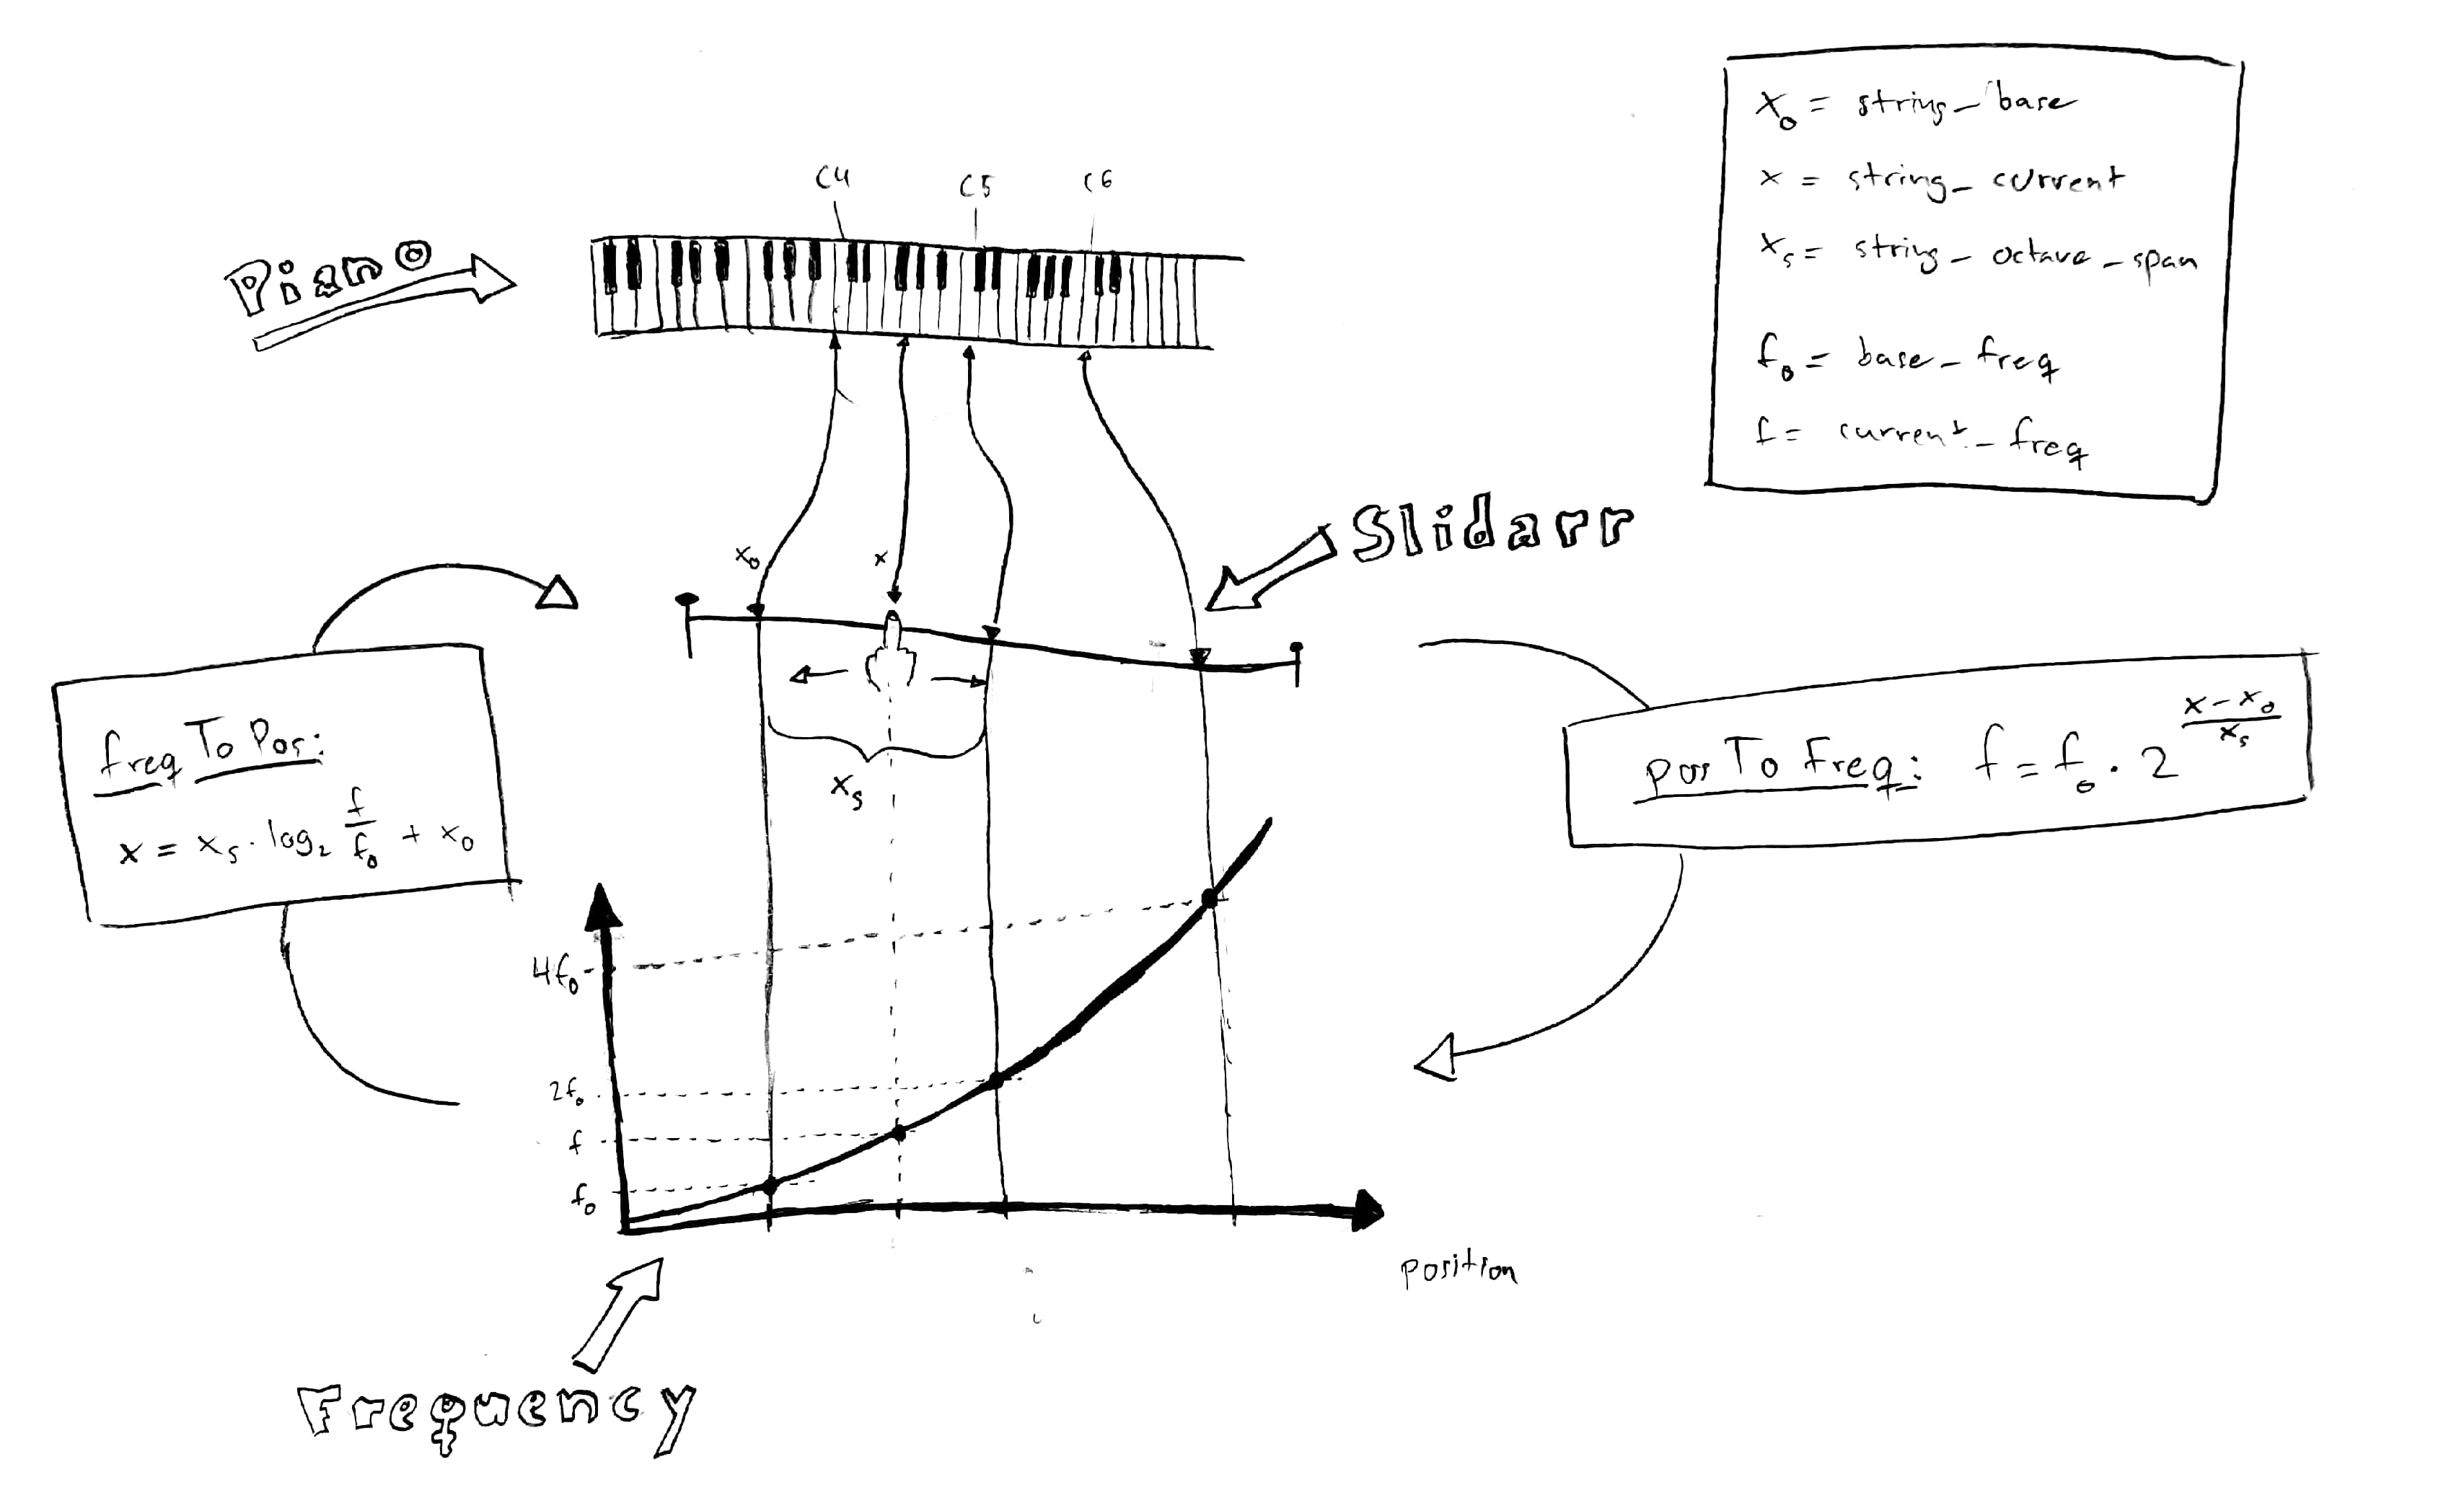
\includegraphics[width=1\textwidth]{slidarr_2_.jpg}
  \caption{slidarr scetch}
  \label{fig:slidarr}
\end{figure}

Blabla blabla bla.

To sum it up these are the major functionalities of the Slidarr and important to know:
\begin{itemize}
 \item Touching, turn specific note on
 \item Sliding, changing the pitch and jumping to another tone
 \item Calibrating, setting the minimum and maximum range on the hardware for one octave
 \item Scrolling, moving the octave on the keyboard to higher or lower tones
\end{itemize}


\section{Analysis}

\subsection{Resistance measurement} \label{sec:resistance_measurement}
One way of determining the finger's position of the string is to measure the resistance from one end of the string to the finger. A copper wire of length 1 meter and diameter of \SI{0.5}{mm} has a resistance of \SI{0.5}{\ohm} per meter \cite{copperresistance}. In order to track the position  with millimeter accuracy, we need to measure in the sub-\si{\milli\ohm} range. 

This can be done in many different ways. One way is using a resistor bridge setup, e.g. a Wheatstone or Kelvin bridge, which is able to sense tiny changes in resistance. However, the bridge needs to be balanced with accurate resistors of similar value of the measured resistor, which is hard to achieve with standard resistors when the measured resistance is this small.

\begin{figure}[ht]
  \centering
  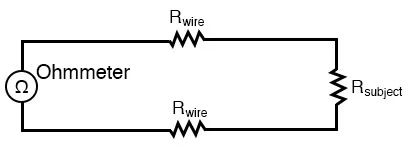
\includegraphics[width=0.5\textwidth]{4-wire-sensing}
  \caption{4-terminal measurement}
  \source{allaboutcircuits.com}
  \label{fig:4terminal}
\end{figure}

An more suitable method is to use four-terminal measurement as shown in figure \ref{fig:4terminal}. A known constant currenti $I$ is fed through the resistor with unknown resistance $R$, and the voltage drop $V$ is measured with a separate pair of wires. The resistance can then easily be calculated using Ohms law, $ R = V / I $.

\subsection{Voltage measurement} \label{sec:voltage_measurement}
Using four-terminal measurement with a current of \SI{100}{\milli\ampere}, the change in voltage per millimeter string is \SI{50}{\micro\volt}. This has now turned into a matter of measuring low-level voltages.

A 12-bit ADC operating at \SIrange{0}{3.3}{\volt} has a resolution of \SI{0.8}{\milli\volt} per bit. The signal needs to be amplified by at least 16 times in order to achieve \si{\milli\meter} accuracy.

\subsubsection{Instrumentation amplifier}
Since we are interested in the voltage difference over the string, a differential amplifier is a good choice for amplifying the signal. The \textit{instrumentation amplifier} is widely used for amplifying low-level signals. It is stable and easy to adjust, since the amplification can be set by a single resistor \cite{in}.

\subsection{The MIDI protocol}
MIDI (Musical Instrument Digital Interface) protocol is the industry standard for communication between electronic musical instruments and synthesizers \cite{midiorg}. It does not transport the audio itself, instead messages with instructions about the note, its volume and duration are sent to a receiving device which generates the sound. 

MIDI was designed to be used with digital piano keyboards. The messages indicate \textit{note on}, \textit{note off}, and their \textit{velocity} (volume). The protocol is built around the concept of piano notes, which is not optimal for the Slidarr since it operates at a continous scale rather than at fixed frequency intervals.

The solution to this is the \textit{pitchbend} message, which is usually controlled by a wheel controller on the keyboard. It is a global parameter that bends the pitch (offsets the frequency) of the currently played notes, on synths that support it. The amount of bending is not standardized and can differ between synthesizers.

The MIDI message consists of three bytes: the \textit{command} and two \textit{parameters} \cite{midistanford}. There are many different commands, but the Slidarr only needs the three as shown in table \ref{table:midi_msgs}.

\begin{table}[h]
  \centering
  \caption{MIDI messages}
  \label{table:midi_msgs}
  \begin{tabular}{llll}
    Action     & Command & Parameter 1 & Parameter 2 \\ \hline
    Note off   & 0x80    & Key         & Velocity    \\
    Note on    & 0x90    & Key         & Velocity    \\
    Pitch bend & 0xE0    & Value       & Value      
  \end{tabular}
\end{table}

\subsection{Standard music notations and frequencies}
An \textit{octave} is a frequency interval where the higher note is twice the frequency of the lower note \cite{octave}. In western music, an octave is divided into 12 \textit{semitones}, named C through B, which correspond to a key on a piano. This is the pattern of keys that repeat over the keyboard as shown in \ref{fig:octave}. A piano usually stretches over seven octaves, numbered 1 through 7. A note needs to be identified by not only its name, but also its octave index, e.g. C4.

\begin{figure}[h]
  \centering
  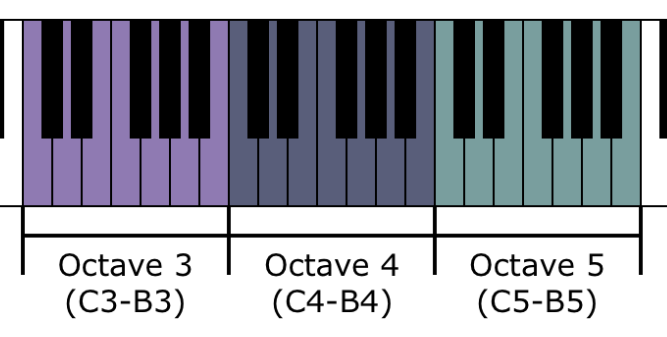
\includegraphics[width=0.5\textwidth]{octaves}
  \caption{Octaves on a piano}
  \source{https://music.stackexchange.com/questions/69410/what-is-an-octave}
  \label{fig:octave}
\end{figure}

Now when octaves, semitones and their relationships have been defined, the final tuning of the piano is left to be decided in order to be able to calculate the frequency of every key of a piano. Typically, the \textit{concert pitch} is used, which specifies that note A4 has a frequency of \SI{440}{\hertz}. All other keys on the piano can be derived from this key.

The MIDI standard specifies that C4 has index 60. Hence, note A4 has index 69. The frequency $f$ for any key $n$ can be calculated using the following formula:

$$ f = 440 \times 2^{\frac{n-69}{12}} $$

\subsection{Sound generation}
The MIDI signals does nothing on their own. They need to be interpreted by a \textit{sound synthesizer}, or \textit{synth} in short, which uses the MIDI input to control the frequency and characteristics of its audio output. They usually provide an interface for adjusting the parameters, making it possible to generate a wide variety of sounds using the same synth. 

There are countless of free software synths available online that supports MIDI and can be used with the Slidarr, but not every sound is suitable for this instrument. Since it is \textit{monophonic}, i.e. it can only play one note at a time, and is able to slide continously between notes, the synth should preferrably have a soft sound with a constant volume in order to hide the transition between notes when sliding.

\section{Design}

\subsection{Hardware}

The hardware can be divided into three parts: the \textit{string sensor}, i.e. the string and the conductor; the \textit{positioning unit}, and the microcontroller.

\subsubsection{Positioning unit}
The positioning unit contains the constant current regulator and the instrumentation amplifier, as described in section \ref{sec:resistance_measurement}. An LM317 voltage regulator is set up to feed a constant current through the string. The current $I$ is determined by resistor $R2$ \cite{lm317}:

$$ I = \frac{1.25}{R_2} $$

For $ I = \SI{100}{\milli\ampere} $, $R_2 = \SI{12.5}{\ohm} $. This resistor also dissipates some power, and a high power resistor is necessary. In the lack of these, 8 parallel \SI{100}{\ohm} \SI{0.25}{\watt} resistors was sufficient.

\begin{figure}[h]
  \centering
  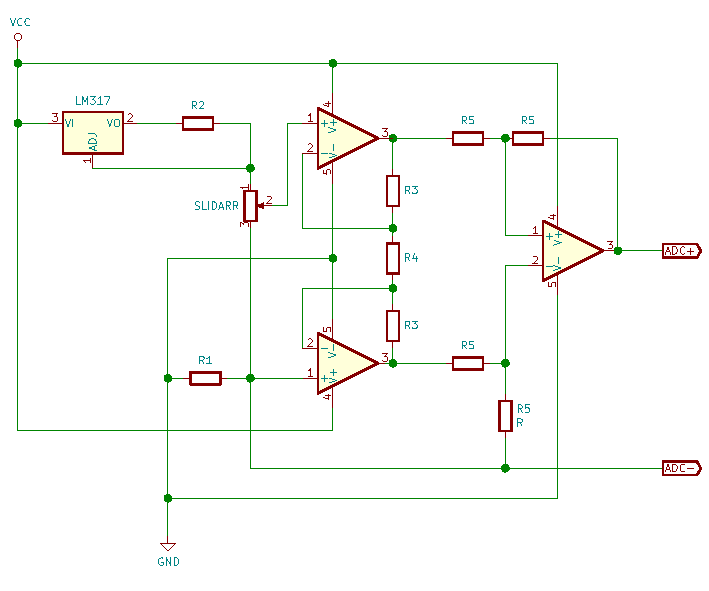
\includegraphics[width=0.9\textwidth]{slidarr-circuit}
  \caption{Positioning unit}
  \label{fig:slidarr-circuit}
\end{figure}

The instrumentation amplifier is built using three operation amplifiers. Its total amplification $A$ can be determined by:

$$ A = 1 + \frac{2R_3}{R_4} $$. 

As mentioned in section \ref{sec:voltage_measurement}, $ A \geq 16 $ for \si{\milli\meter} resolution. But even higher precision be achieved. The maximum voltage difference over the string is:

$$\SI{300}{\milli\meter} \cdot \SI{15}{\micro\volt}= \SI{15}{\milli\volt} $$. 
The resolution is maximized when the maximum amplification is \SI{3.3}{\volt}. The amplification then becomes:

$$ A = \SI{3.3}{\volt} / \SI{15}{\milli\volt} = 220 $$ 

By choosing $R_3 = \SI{10}{\kilo\ohm} $ and $R_4 = \SI{100}{\ohm} $, $ A = 201 $ which is more than sufficient.

Since the op-amps need to be powered with both positive and negative voltage, relative to the input voltage, the resistor $R_1$ is used to raise the string sensor's voltage to $V_{CC}/2$.

The TS464 is a chip with four integrated op-amps. Figure \ref{fig:slidarr-circuit2} shows how the final circuit is set up using this chip.

\begin{figure}[h]
  \centering
  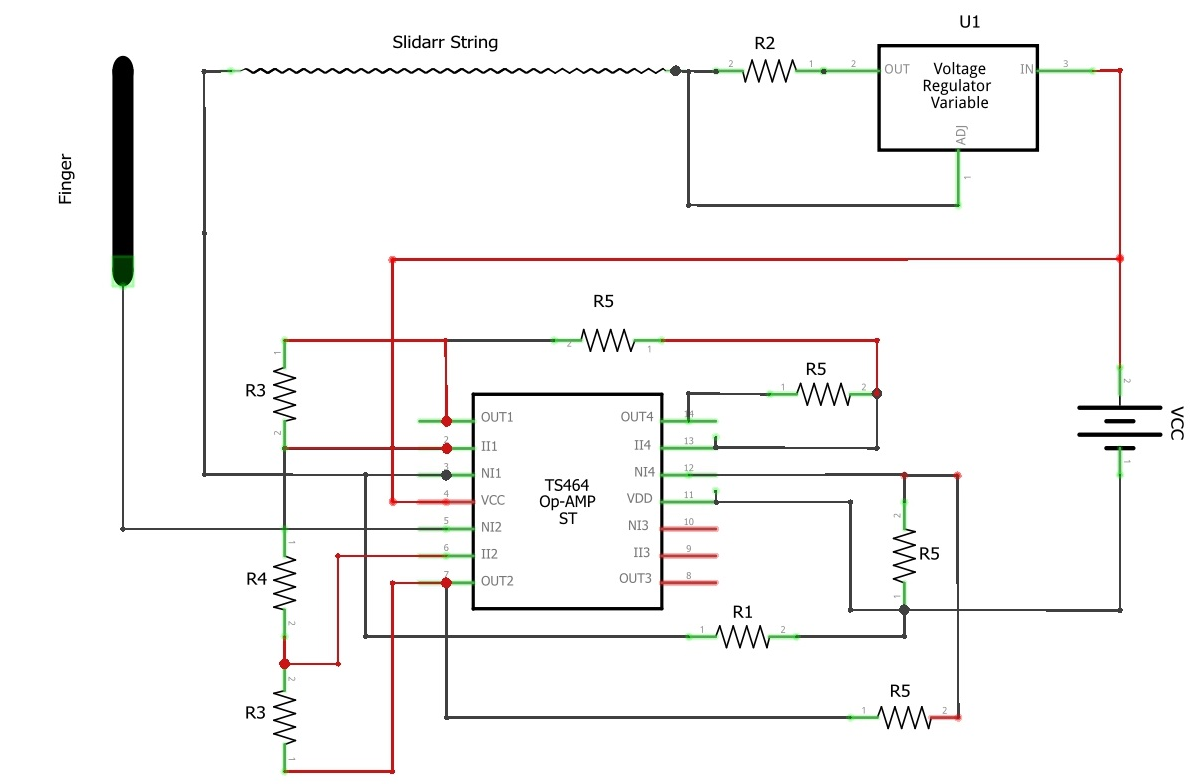
\includegraphics[width=0.9\textwidth]{slidarr-circuit2}
  \caption{The positioning unit using a TS464 quad-op-amp.}
  \label{fig:slidarr-circuit2}
\end{figure}

\subsubsection{String sensor}
The string sensor consists of a \SI{300}{\milli\meter} long copper wire with a diameter of \SI{0.5}{\milli\meter}, stretched between two screws on a wooden plank (see figure \ref{fig:string_sensor}.  The user wears a conductive copper C-shaped ring on one of its fingers, which will be used to make contact with the string. The C-shape makes it possible to bend the ring to a perfect fit for the user. The voltage difference can then be measured between the ring and one end of the string. The string sensor can be though of as a simple potentiometer, marked SLIDARR in figure \ref{fig:slidarr-circuit}.

\begin{figure}[h]
  \centering
  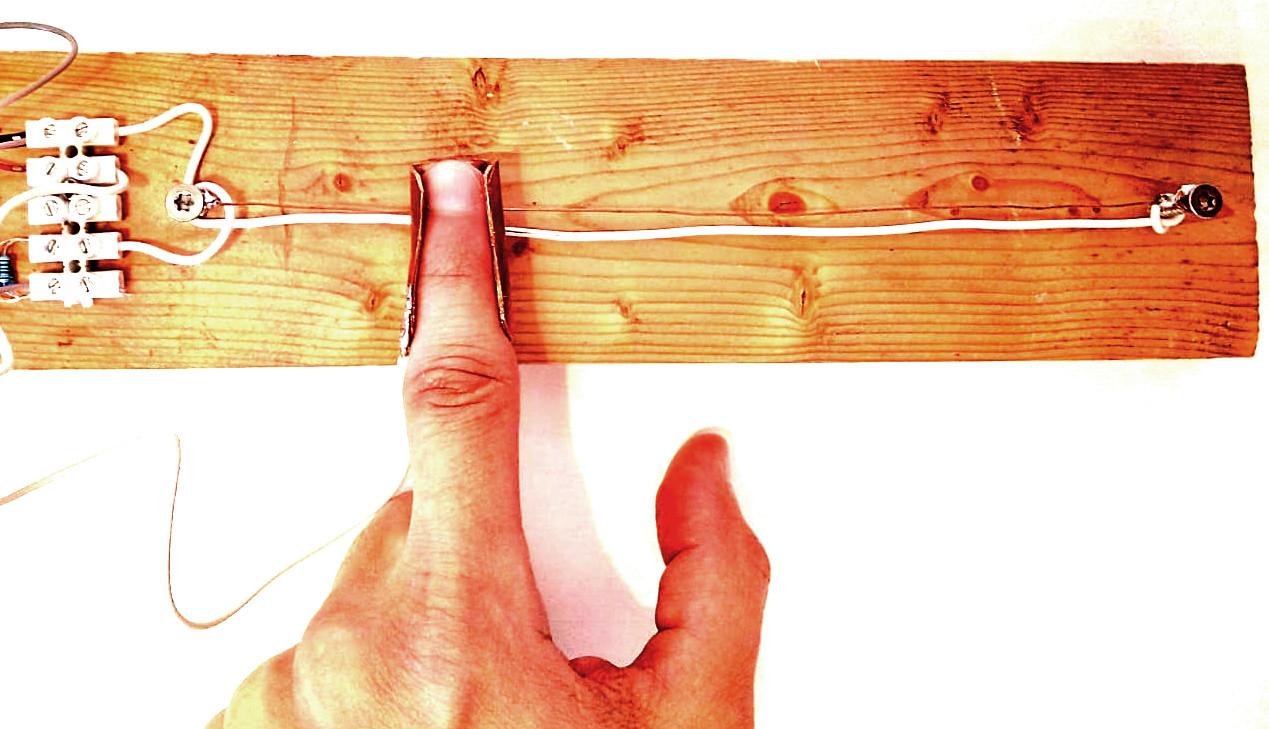
\includegraphics[width=0.9\textwidth]{string-sensor}
  \caption{The string sensor}
  \label{fig:string_sensor}
\end{figure}

\subsubsection{Power supply}

\subsubsection{Microcontroller}

\section{Implementation}

\subsection{System overview}
For the total system to play music in the end, there are four major parts: the circuit/instrument itself, the microcontroller with its peripherals, the connection to the synthesizer/computer and the synthersizer/computer. See image x.

\begin{figure}[ht]
  \centering
  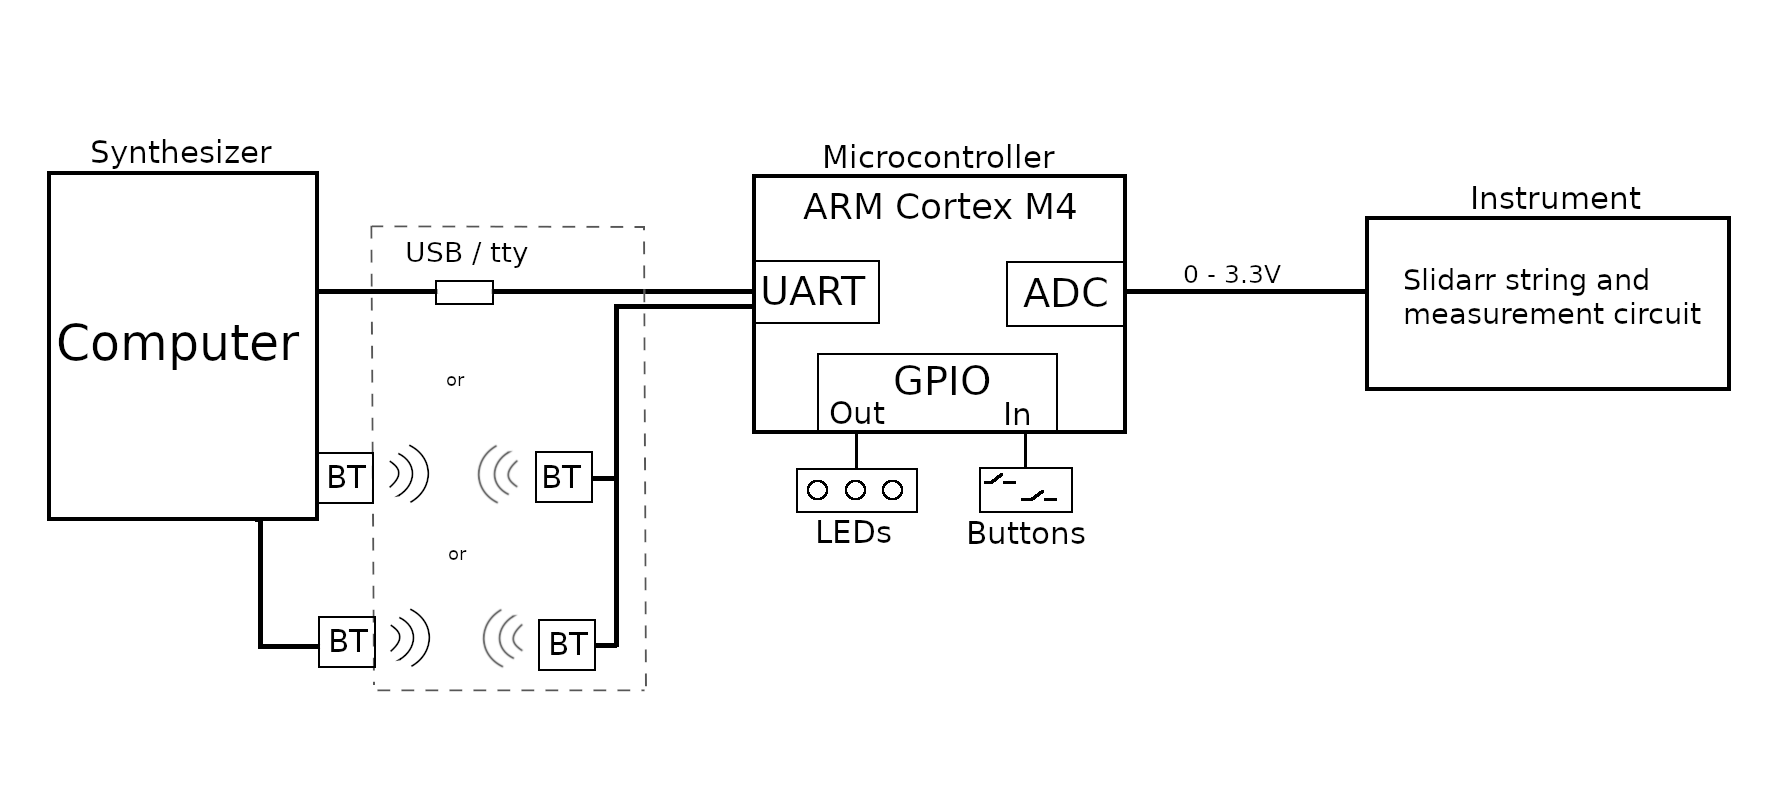
\includegraphics[width=1\textwidth]{BasicSystemOverview.png}
  \caption{slidarr overview}
  \label{fig:slidarr overview}
\end{figure}

The microcontroller is an ARM Cortex-M4 (TI TM4C123GH6PM for the prototype) that is running at 16MHz. The connection to the computer or snythesizer is optionally either via a tty to USB converter, Bluetooth directly or a Bluetooth bridge with a USB compatible end device.

\subsection{Peripherals}
Peripherals used are the on-chip 12-bit ADC, General Purpose Inputs/Outputs and the UART.

The analog to digital converter is 12-bit wide and the used reference voltage is the same as the microcontroller is using (3.3V). Using the above described measurement method the voltage difference from the low end of the string to the upper end lies between 0.2V to 0.4V. With a step size of 0.8mV this gives us at least 250 steps to work with per octave depending on the calibration. The ADC reads only one sample at a time from a single channel and the conversion is triggered by software when needed.

There are two inputs used. The two inputs are buttons, that put the device into calibration mode and into scrolling mode. For the buttons internal on-chip pull-ups are enabled so that no additional components are needed other than the button. The buttons are debounced in the software.

Three outputs are connected to three LEDs of different colors by using transistors as switches and resistors to limit the current. The green LED indicates if the string is touched at the moment. The red LED signals if the calibration mode is currently running. The blue LED shows when the user is in the scrolling mode.

The UART is used to send out the MIDI bytes to the sound generating device. Only the transmit line is utilized. The receive line stays untouched for the forseeable future because there is no use for it at this stage. The UART is configured for 8 bits with baud rates of 9600, 38400 or 115200 which can be changed in the defaults.h file. The chip has a 16 byte transmit buffer that is implemented into the hardware. This makes it easy to send out multiple bytes (3 bytes for midi messages) putting them into the buffer all at once without having to wait for every single byte to be transmitted, which would block the execution otherwise.

\subsection{Programming model}
The microcontroller is programmed `bare-metal` so to say. This means there is no use of external libraries and the configuration of the peripherals are all made with the help of the reference manual setting the registers directly. The only thing that is used, is the given header file for the microcontroller.

The code starts initializing most of the used variables on the stack locally in the main function. A defaults header file exists where parameters for the configuration can be changed. Then all the peripherals and the buffer, to keep the history of the ADC values, are initialized. Finally the code enters into a state machine and stays there.

\subsection{The state machine}

The state machine runs in an infinite while loop that is controlled by the SysTick timer. The timer can be set at a specified interval given by the defaults. A five milliseconds interval is a good value to use because it gives the processor enough time to do all the calculations and doesn't spam the UART too much while not creating a noticeable delay (respecting the buffer). After the code does all the processing it waits for the SysTick timer to timeout and repeat the process. The waiting is blocking the processor which is intended and doesn't harm the implementation at the current stage.

There are four states the slidarr is in at any given point in time which are IDLE, SLIDE, SCROLL and CALIBRATE. See image x. There are three LEDs which are turned on when entering the states of SLIDE, SCROLL and CALIBRATE to give the user feedback of the devices state which have the colors green, blue, and red respectively.
The states are influenced by the following properties: string touched flag, string sliding flag, pitchbend maximum offset, calibration button and scrolling button.

\begin{figure}[ht]
  \centering
  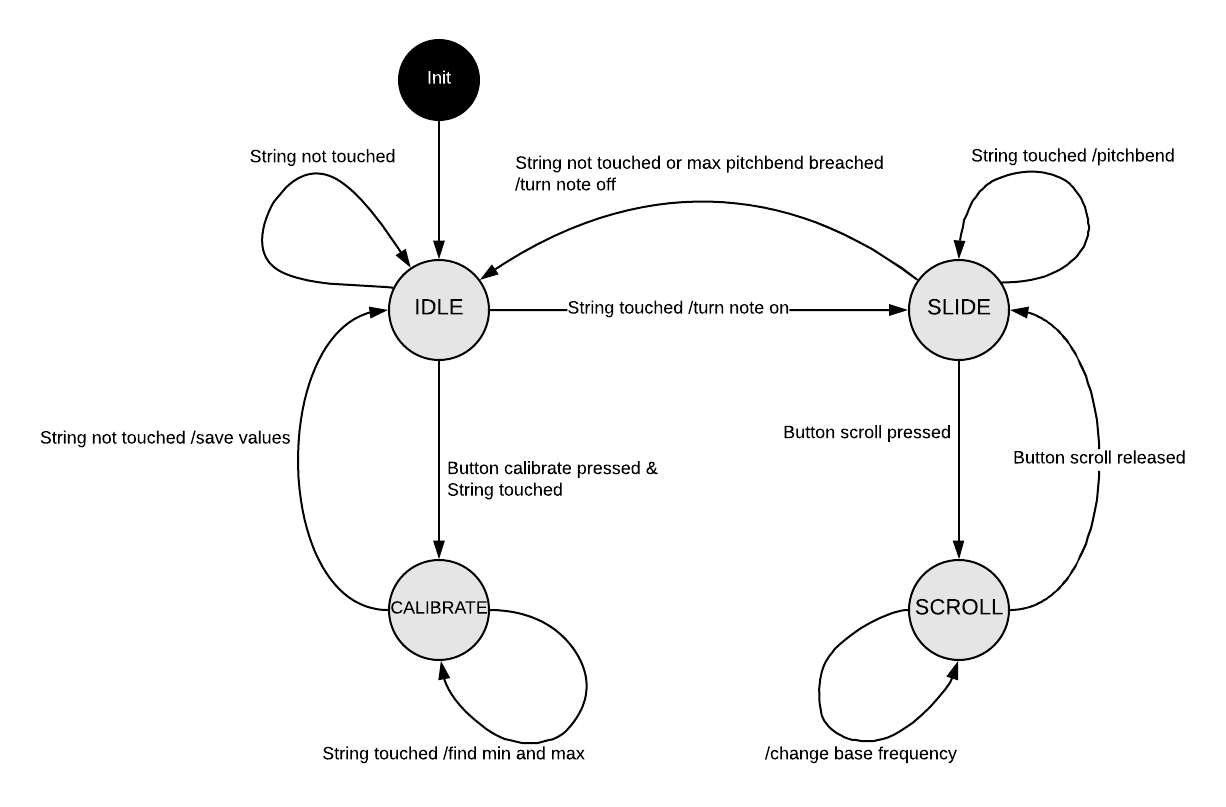
\includegraphics[width=1\textwidth]{SlidarrStateMachine.png}
  \caption{Slidarr state machine}
  \label{fig:slidarr state machine}
\end{figure}

\subsection{ADC sample buffering}
The flags of string touched and string sliding are set by a mean and standard deviation calculated from the last n samples from the ADC. The mean and standard deviation filter the sampled values from noise and keep the slidarr from jumping around too much.
Every read from the ADC is put into a ring buffer of a specified size by the defaults that keeps the history. The size depends on the sample time and noise, but recommended sizes range from 5 to 50 values. Having a large sample time and a big history buffer will result in larger delays and response time.

To set the flags there are treshold values that are compared to the mean and standard deviation to decide the state.

\subsection{Calibration}
The strings needs to be calibrated to find out at what voltage the string starts and where it ends. To start the calibration the calibration button is pressed without releasing it. Only when both the button and the string is touched will the calibration start. After the string is touch the button can be released. Sliding from the minimum to the maximum or vice versa will find the string base value (min) and the string octave span (min - max). Removing the contact from the string ends the calibration. The area that was slid over represents one octave afterwards.

\subsection{Scrolling}
While sliding it is possible to change the current octave to a higher or lower one by scrolling. When the scroll button is pressed while sliding it will change the base frequency to a higher or lower depending on the sliding direction.

\subsection{Making MIDI continuous / bitchbending}
To play a tone with MIDI every note has to be turned on and off manually. In addition to just playing the note it has a frequency offset that is sent by a pitchbend message. To get the sliding effect a note needs to be turned on and depending on the location the offset will need to be set. When sliding this offset changes and has to be continously transmitted. Sliding over to a another note (passing the maximum pitchbend), the old note has to be turned off and the new note be turned on, sending the offset from the point of view of the new note.

\subsection{Wireless Connection}
\paragraph{}In this project, a Bluetooth module HC-05 is used as a second transmitting device together with USB-TTL device, the advantage of using a wireless connection other than moving the microcontroller around freely within the area of the network, it gives the ability to test the output signal on different software. Also, these two ways of transmitting the MIDI message improved the testing process. 

The Bluetooth module HC-05, it operates on 5 V, supports Bluetooth 2.0 and communicates via UART. Both Bluetooth modules have configured at baud rate from default 9600 to 115200 by AT command mode, as well as one of the module configured as master (it only connect to the slave module) and other one left as a slave.

There are two ways of sending MIDI note from TM4C microcontroller, one way is through a direct connection between the microcontroller with Bluetooth module and the host computer that support Bluetooth connection (paired Bluetooth device). The second alternative way is preferable as this actually not involve any third-party software in the host computer, through a wireless bridge link between the TM4C microcontroller and Arduino-Micro microcontroller together by using master and slave Bluetooth module. Both methods of implementation are briefly explained in details.
\subsubsection{Direct Bluetooth Connection}
\paragraph{}A Bluetooth slave connected with the microcontroller and after the pairing process in the host computer (pairing only made once) than Bluetooth Led state change from blink every second to stop blinking. The host computer will act as a central hub, and it is as simple as a two-click process.

In this connection, two software required LoopMIDI [7] and the Hairless MIDI [8] together. The LoopMIDI software created a virtual loopback MIDI-ports that can be recognized in synthesizer software, while the Hairless MIDI change the serial port over Bluetooth link to a MIDI output which is the created port in LoopMIDI software. 

The software is periodically checked and if any MIDI note received, the synthesizer will generate audio signals.

\subsubsection{Wireless Bridge Connection}
\paragraph{}A Bluetooth slave and master connected to the TM4C and Arduino-Micro microcontroller respectively. Arduino-Micro and few other Arduino are supported because it has HID (Human Interface Devices) capability, this microcontroller used because it supports MIDIUSB library [9] that allows the transmitted message to be easily recognized by any synthesizer software, unlike the the first way which used third-party software in the host computer. The two Bluetooth modules will connect to each other as long as the signal is not out of range, and it is a plug-and-play process.

In this connection, the Arduino-Micro will receive the MIDI messages from the wireless connection and send it back to the host computer through the serial port (USB). 

\section{Testing and debugging}
The Slidarr has been developed in a modular approach, adding the functionalities together one by one, until the end when testing the system as a whole. The system is tested empirically, going through all the use cases, treating the device as a black box.

Using the debugger to view the memory during faulty behaviour was enough to find the bugs and misbehaviour. Instead of using the whole Slidarr hardware (string, circuit, power supply, etc) to test the software, a simple potentiometer with a button connected to the ADC, similar behaviour could be simulated.

Due to the instrument not being used in a safety critical system there is no further need for more advanced testing and verification at this stage of the project.

\section{How to use (for powerpoint and demo, remove this later on)}
-how to connect
-make simple tone
-make calibration
-bend pitch
-scroll

\section{Results}

\subsection{Conclusion}
Being a prototype, the Slidarr is a viable instrument very capable of creating music in the hands of an artist.

\subsection{Future improvements and implementations}
As the Slidarr proved to be successful, many things can now be done to make Slidarr more accessible to the public and make it a popular instrument one day. These improvements are both on the hardware side and software side.

The code can be made more modular for use on other microcontrollers, for example by converting it to use CMSIS. A more optimal and cost effective microcontroller can be choosen. The current program uses 12KB (out of 256KB) of flash storage and 500 bytes (out of 32KB) of SRAM. In addition the software runs without any problems at 16MHz. This means a much smaller microcontroller could be used for future implementations.

Along with choosing a smaller microcontroller a more visually appealing, compact, and battery powered device can be construted. Using higher precision ADCs and other materials that have other eletric conductivity properties to measure the distance can be researched for use in different instrument variations.

The use of multiple strings controlling e.g. the velocity and volume can be implemented. The type of instrument that can be created after this point is only limited by the imagination of the reader blabla

picture with concepts

\newpage
\begin{thebibliography}{9}

\bibitem{copperresistance} 
Chemandy Electronics: Round Wire Resistance Calculator,
\\\texttt{https://chemandy.com/calculators/round-wire-resistance-calculator.htm}

\bibitem{in} 
Electronics Hub: Instrumentation Amplifier Basics and Applications,
\\\texttt{https://www.electronicshub.org/instrumentation-amplifier-basics-applications}

\bibitem{midiorg} 
The MIDI Association,
\\\texttt{https://www.midi.org}

\bibitem{midistanford}
Stanford CCRMA: Essentials of the MIDI protocol,
\\\texttt{https://ccrma.stanford.edu/~craig/articles/linuxmidi/misc/essenmidi.html}

\bibitem{octave}
Encyclopedia Britannica: Octave,
\\\texttt{https://www.britannica.com/art/octave-music}

\bibitem{sengpielaudio}
Sengpiel Audio: Keyboard ad frequencies,
\\\texttt{http://www.sengpielaudio.com/calculator-notenames.htm}

\bibitem{lm317}
LEDnique: LM317 constant-current power supply,
\\\texttt{http://lednique.com/power-supplies/lm317-constant-current-power-supply/}

\bibitem{loopmidi}
Virtual loopback MIDI software,
\\\texttt{https://www.tobias-erichsen.de/software/loopmidi.html}

\bibitem{sengpielaudio}
The Hairless MIDI Serial Bridge Software,
\\\texttt{https://projectgus.github.io/hairless-midiserial/}

\bibitem{sengpielaudio}
Arduino Libraries: MIDIUSB library over USB,
\\\texttt{https://github.com/arduino-libraries/MIDIUSB}

\end{thebibliography}

\newpage
\begin{appendices}

\section{Some stuff}

\section {More stuff}

\end{appendices}


\end{document}
